\documentclass[12pt]{article}
\linespread{1.3}
\usepackage[T1]{fontenc}
\usepackage{polski}
\usepackage[utf8]{inputenc}
\usepackage{geometry}
\usepackage{graphicx}
\usepackage{enumitem}
\usepackage{textcomp}
\usepackage{hyperref}
\usepackage{subcaption}
\usepackage{caption}
\usepackage{graphicx} 
\usepackage{float}
\usepackage{xurl}
\usepackage{xcolor}

\usepackage{lscape}

\newgeometry{tmargin=3cm, bmargin=3cm, lmargin=3cm, rmargin=3cm}

\begin{document}

\begin{titlepage}
	\center
	
	
	%--------------  NAGŁÓWKI ---------------------------------------------------------
	
	\textsc{\Large Politechnika Wrocławska}\\[0.5cm] % Name of your university/college
	\textsc{\large Wydział Elektroniki}\\[5cm] % Major heading such as course name
	
	%--------------  TYTUŁY   ---------------------------------------------------------
	
	\textsc{\LARGE PROJEKT ZESPOŁOWY}\\[2cm] % Minor heading such as course title
	{ \Large \bfseries GarageAssistant}\\[4cm] % Title of your document
	%--------------  TERMIN ZAJĘĆ -----------------------------------------------------
	\begin{minipage}{0.83\textwidth}
	\begin{flushleft} \large
	Termin zajęć: Środa, 13-16 \\[2cm]
	\end{flushleft}
	\end{minipage}
	\\[2cm]
	
	%--------------  AUTORZY  ---------------------------------------------------------
	
	\begin{minipage}{0.4\textwidth}
	\begin{flushleft} \large
	\emph{Autorzy:}\\
	Marcin \textsc{Bober}\\
	Janusz \textsc{Domaradzki}\\
	Michał \textsc{Kowalski}\\
	\end{flushleft}
	\end{minipage}
	~
	\begin{minipage}{0.4\textwidth}
	\begin{flushright} \large
	\emph{Prowadzący zajęcia:} \\
	dr inż. Krzysztof \textsc{Arent} 
	\end{flushright}
	\end{minipage}\\[1cm]
	
	%--------------  DATA     ----------------------------------------------------------
	
	{\large Wrocław, \today}\\[1cm]
	
	\vfill 
	\end{titlepage}


\tableofcontents

\clearpage

\section{Mikrokontroler}

\begin{figure}[H]
	\centering
	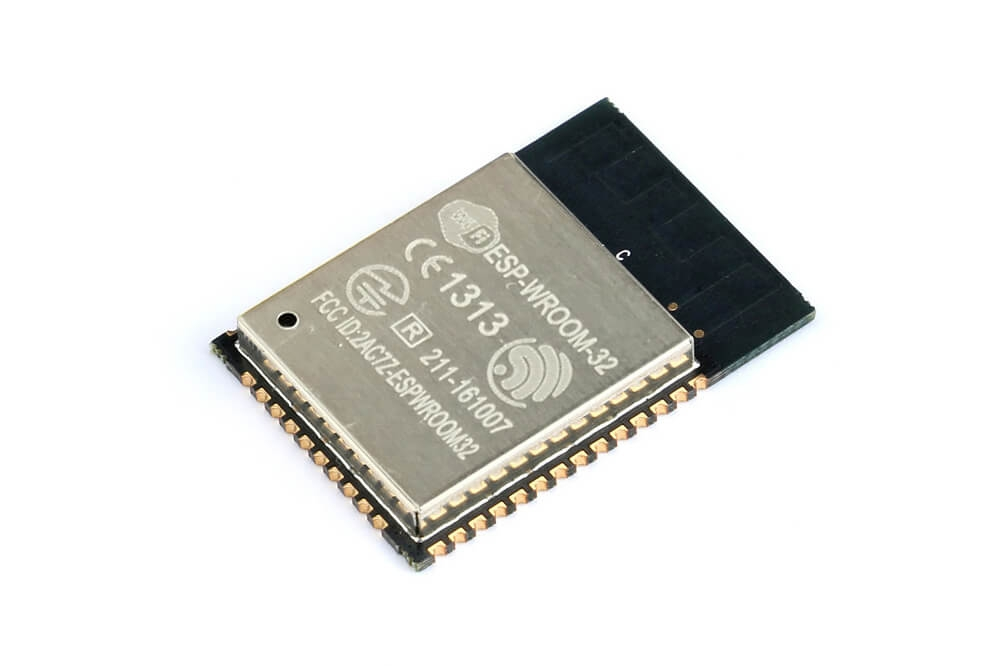
\includegraphics[width=0.6\textwidth]{figures/esp32.jpg}
	\caption{ESP32 WROOM-32}
	\label{fig:mcu}
\end{figure}

ESP32 jest to topowy układ SoC chińskiego producenta Espressif Systems.
Został on wybrany ze względu na zintegrowany modół WiFi i niską cenę.
Wersja WROOM-32 charkteryzuje się:

\begin{itemize}
    \item CPU: Xtensa dual-core 32-bit LX6 microprocessor o taktowaniu 240 MHz.
    \item Ultra low power (ULP) co-processor.
    \item Wi-Fi: 802.11 b/g/n
    \item Bluetooth: v4.2 BR/EDR i BLE
    \item Aktualizacje oprogramowania poprzez sieć
    \item Pamięć Flash: 4 MB
\end{itemize}

\section{Czujniki}
\subsection{HC-SR04}
\begin{figure}[H]
	\centering
	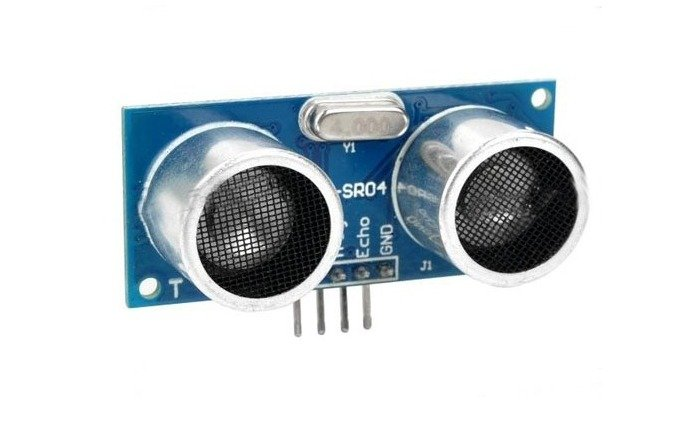
\includegraphics[width=0.5\textwidth]{figures/HC-SR04.jpg}
	\caption{HC-SR04}
	\label{fig:HC-SR04}
\end{figure}

Czujnik ultradźwiękowy działający w zakresie 2-200 cm.
Jest to główny czujnik wykrywający nadjeźdzający pojazd od przodu.

\begin{itemize}
    \item Napięcie zasilania: 5 V
    \item Średni pobór prądu: 15 mA
    \item Zakres pomiarowy: od 2 cm do 200 cm
    \item Częstotliwość pracy: 40 kHz
\end{itemize}

\section{Zasilanie}
\subsection{STUSB4500}

\begin{figure}[H]
	\centering
	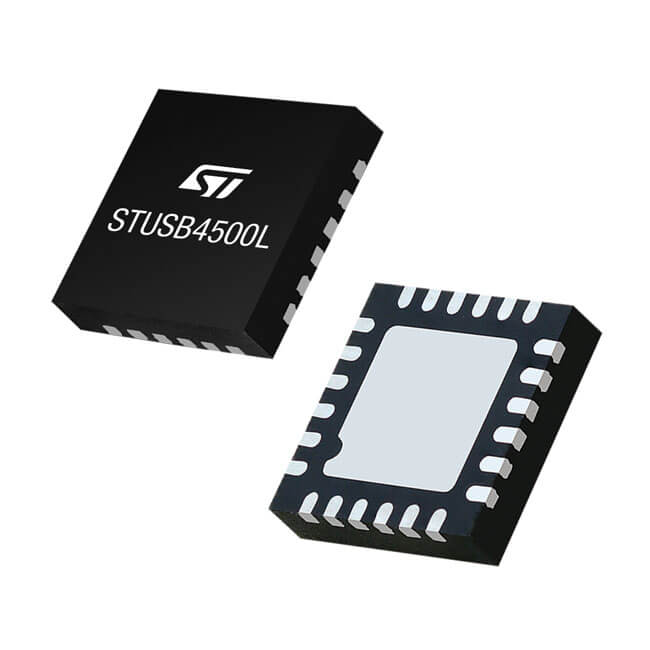
\includegraphics[width=0.5\textwidth]{figures/stusb.jpg}
	\caption{STUSB4500}
	\label{fig:stusb}
\end{figure}

Energii do urządzenia dostarczać będzie kontroler zasilania USB 
STUSB4500 \cite{STUSB4500f}. Obsługuje on technologię "USB power delivery", 
co 

\begin{itemize}
    \item wykrywanie dołączenia zasilania do portu USB-C
    \item zestawienie poprawnego połączenia źródła energii i odbiornika
    \item obsługa obracania wtyczki i skrętu żył kabla dla zapewnienia poprawnego przekazywania danych (MUX control)
    \item negocjacja warunków zasilania zgodnie z power delivery
    \item konfigurowanie zasilania z szyny VBUS oraz monitorowanie stanu tej linii
    \item realizacja zabezpieczeń przed przepięciami i zbyt dużym napięciem zasilania
\end{itemize}


\section{Informacja dla kierowcy}

\subsection{Pasek led}
\begin{figure}[H]
	\centering
	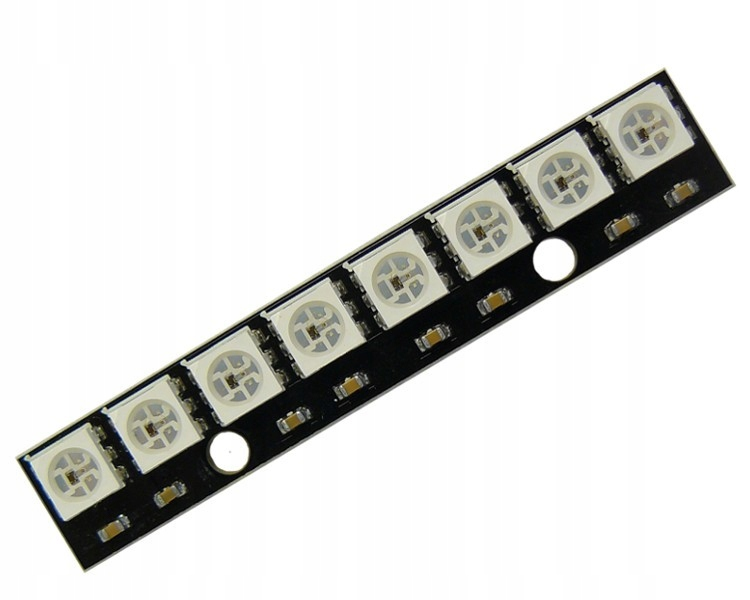
\includegraphics[width=0.5\textwidth]{figures/ws2812.jpg}
	\caption{WS2812}
	\label{fig:ws2812}
\end{figure}
Aby kierowca mógł z łatwością ocenić odległość od ściany, system będzie
wyposarzony w oświetlenie ledowe informujące o pozostałym odstępie.
Będzie ono bazować na diodach WS2812.

\subsection{Buzzer}
\begin{figure}[H]
	\centering
	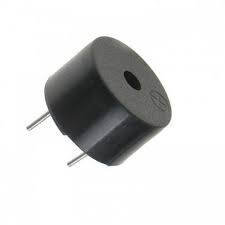
\includegraphics[width=0.5\textwidth]{figures/buzzer.jpg}
	\caption{buzzer}
	\label{fig:buzzer}
\end{figure}
Dodatkowym aspektem informacyjnym będzie sygnał dzwiękowy generowany
przez buzzer magnetyczny.

\section{Inne}
\begin{itemize}
    \item Wyświetlacz OLED
    \item Przyciski
    \item Diody led
    \item stabilizator napięcia 3.3V
    \item kondensatory filtrujące
    \item tranzystor NPN
    \item dioda odsprzęgająca
\end{itemize}

\begin{thebibliography}{99}
\bibitem{STUSB4500f} https://www.st.com/en/interfaces-and-transceivers/stusb4500.html
\end{thebibliography}

\end{document}
